游戏开发是软件工程中最有趣的话题之一。C++因其高效而广泛应用于游戏开发中,但由于言没有GUI组件,所以在后端使用。本章中,我们将学习如何在后端设计策略游戏。我们将把前面章节中学到的所有东西都结合起来,包括设计模式和多线程。 \par
我们要设计的游戏是一款名为《读者与扰乱者》的策略游戏。玩家创造了能够建造图书馆和其他建筑的单位,也就是所谓的“读者”,以及守卫这些建筑不受敌人攻击的士兵。 \par
本章中,我们将了解以下内容: \par

\begin{itemize}
	\item 游戏制作入门
	\item 深入研究游戏设计过程
	\item 使用设计模式
	\item 设计游戏循环
\end{itemize}

\noindent\textbf{}\ \par
\textbf{编译器要求} \ \par
g++编译器需要添加编译选项 \texttt{-std=c++2a} 来编译本章的代码。可以从这里获取本章的源码文件:https:/​/github.​com/PacktPublishing/Expert-CPP \par

\noindent\textbf{}\ \par
\textbf{游戏制作入门} \ \par
这章中,我们将设计一款策略游戏的后端,玩家可以创建单位(工人,士兵),建造建筑,并与敌人战斗。设计一款游戏,无论是战略游戏还是第一人称射击游戏,都有一些基本元素是相同的,比如:游戏物理元素,能够让玩家觉得游戏更真实,更有沉浸感。 \par
游戏设计中有些组件会在所有游戏中重复出现,如:碰撞检测机制、音频系统、图像渲染等。设计游戏时,我们既可以区分引擎和游戏,也可以开发一个紧密结合的应用程序,将引擎和游戏作为单独的成果。单独设计的游戏引擎,需要允许为进一步开发进行扩展,甚至用于其他游戏。毕竟,游戏都有相同的机制和流程。他们的不同之处在于情节主线。 \par
设计游戏引擎时,应该仔细规划使用该引擎的游戏类型。独立于游戏类型之外,3D射击游戏和策略游戏也有区别。策略游戏中,玩家在一个大的游戏场地上,有策略地部署单位。游戏世界是以自上而下的视角呈现的。 \par

\noindent\textbf{}\ \par
\textbf{了解《读者与扰乱者》游戏} \ \par
这款游戏很简单:玩家拥有有限的资源。这些资源可以用来为游戏角色创造建筑。我们将角色单位命名为读者和士兵。读者是建造图书馆和其他建筑的人物。每个构建的库最多可以容纳10个读者。如果玩家将10个读者移进图书馆,在一段特定时间后,图书馆将产生1个教授。教授是一个强大的单位,可以摧毁三个敌人。教授可以为士兵创造更好的武器。 \par
游戏一开始有一座已经建好的房子,两个士兵和三个读者。一所房子每5分钟生产一个新的读者。读者可以建造新的房子,这样就能产生更多的读者。他们也可以建造兵营来生产士兵。 \par
玩家的目标是建立5个库,每个库至少有一个教授。玩家必须在游戏中保护他/她的建筑和读者不受敌人攻击。敌人称为干扰者,因为他们的目标是干扰读者在图书馆里学习。 \par

\noindent\textbf{}\ \par
\textbf{战略游戏组件} \ \par
我们的策略游戏将包含基本组件——读者和士兵(称为单位)、建筑和地图。游戏地图包含游戏中每个对象的坐标。我们将讨论一个更轻版本的游戏地图。现在,让我们利用设计技能分解游戏本身. \par
游戏由以下角色单位组成: \par

\begin{itemize}
	\item 读者
	\item 士兵
	\item 教授
\end{itemize}

它还包括以下建筑物: \par

\begin{itemize}
	\item 图书馆
	\item 房子
	\item 兵营
\end{itemize}

现在,让我们讨论游戏中每个组件的属性。游戏角色有以下属性: \par

\begin{itemize}
	\item 生命值(整数,每次敌人攻击后会减少)
	\item 攻击力(整数,可以对敌人单位造成的伤害)
	\item 角色(读者,士兵,教授)
\end{itemize}

生命值应该有一个基于单位类型的初始值。例如,读者的初始生命值是10,而士兵的初始生命值是12。当在游戏中,所有的单位都可能受到敌人单位的攻击。每次攻击描述为生命点的减少。我们将减少的生命点数是基于攻击者的攻击力。例如,士兵的攻击力设置为3,这意味着士兵的每一次攻击都会让生命值减少3点。当受攻击的单位生命值小于等于0时,单位将死亡。 \par
建筑也是如此。建筑物有一个建造周期,一个建筑物也有生命值,任何敌人对建筑造成的伤害都会降低这些生命值。以下是建筑物业的完整列表: \par

\begin{itemize}
	\item 生命值
	\item 建筑类型
	\item 建造时间
	\item 生产时间
\end{itemize}

生产单位持续时间是指,生产一个新角色单位所需要的时间。例如,一个兵营每3分钟产生一个士兵,一个房子每5分钟产生一个读者,一个图书馆在10个读者进入图书馆时立即产生一个教授。 \par
现在定义了游戏组件,让我们来讨论它们之间的交互作用。 \par

\noindent\textbf{}\ \par
\textbf{组件之间的相互作用} \ \par
游戏设计的下一个重要内容是角色之间的互动。我们已经提到,读者可以建造建筑物。游戏中,这一过程应该得到重视,因为每种类型的建筑都有其建造时间。因此,如果读者正忙于构建过程,我们应该计算时间,以确保构建将在指定的时间后完成。然而,为了让游戏变得更好,我们应该考虑到不止一个读者可以参与到构建过程中。这应该会使建造楼房的速度加快。例如,如果一个兵营是一个读者需要5分钟建造的,那么两个读者就应该在2.5分钟完成,以此类推。这是游戏中复杂互动的一个例子,可以用下图来描述: \par

\begin{center}
	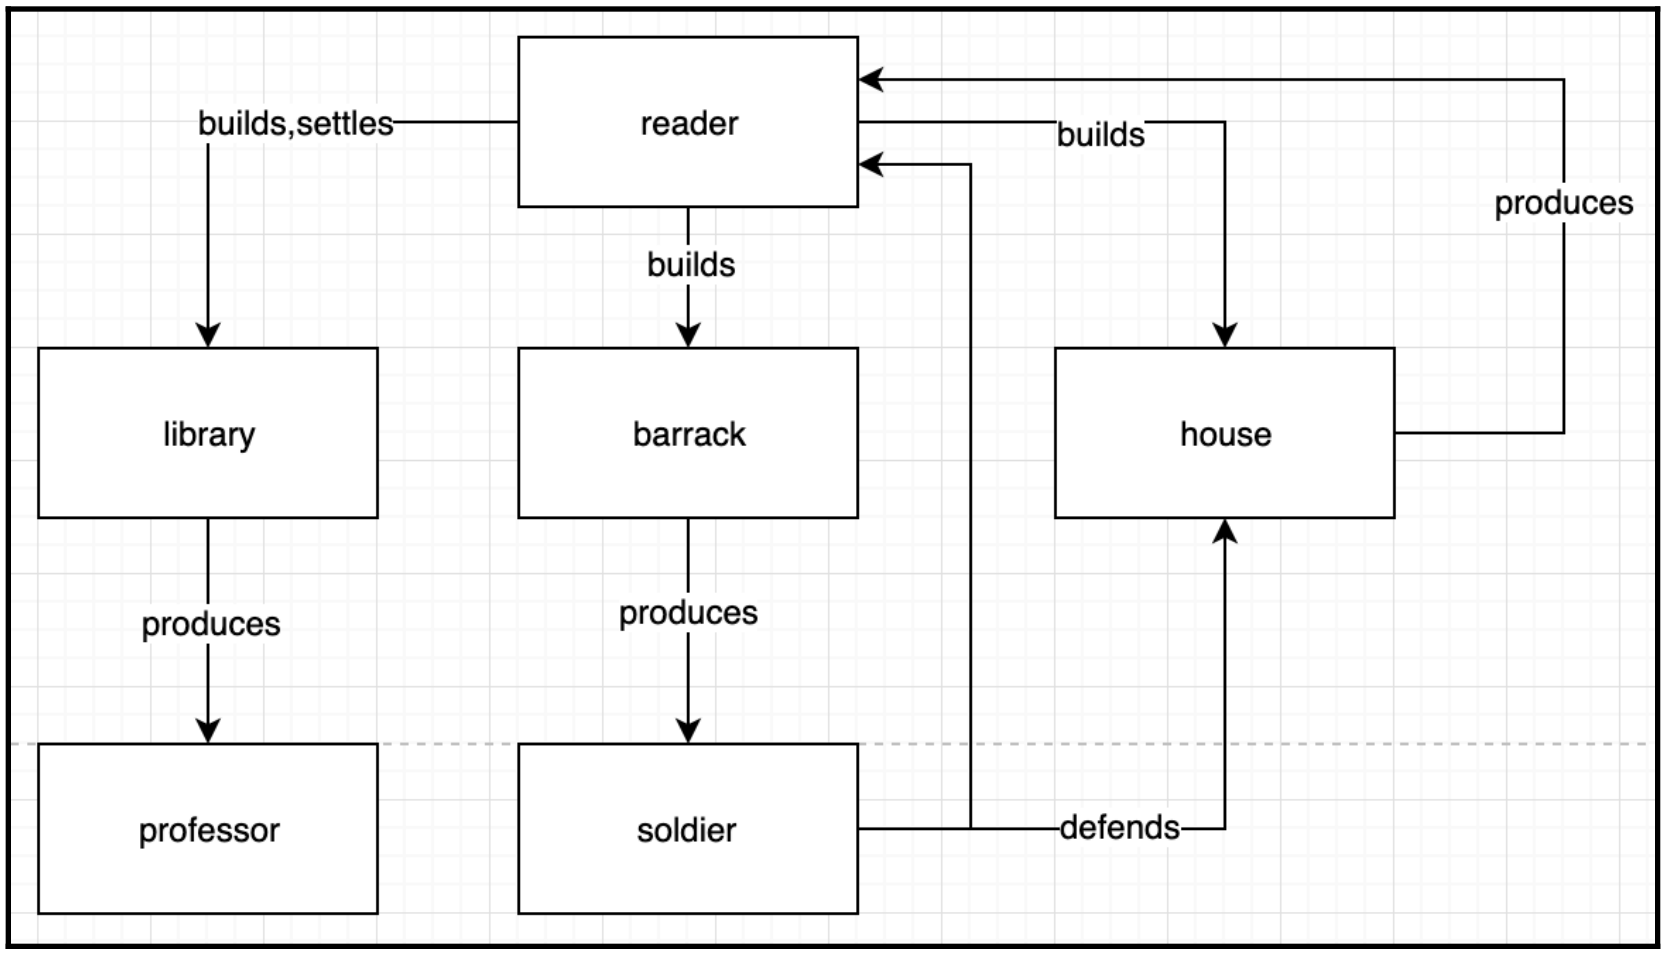
\includegraphics[width=1.0\textwidth]{content/Section-2/Chapter-11/1}
\end{center}

接下来是处理攻击。当一个单位遭受攻击时,我们应该减少单位的生命值。单位可以进行反攻(保护自己)。当有多个攻击者或防御者时,我们应该应该对每次攻击都进行处理。还定义单位每次命中的持续时间,一个单位不应该快速攻击另一个单位。为了让事情更自然,我们会在每次点击之间引入1秒或2秒的暂停。下图描述了一个简单的攻击交互: \par

\begin{center}
	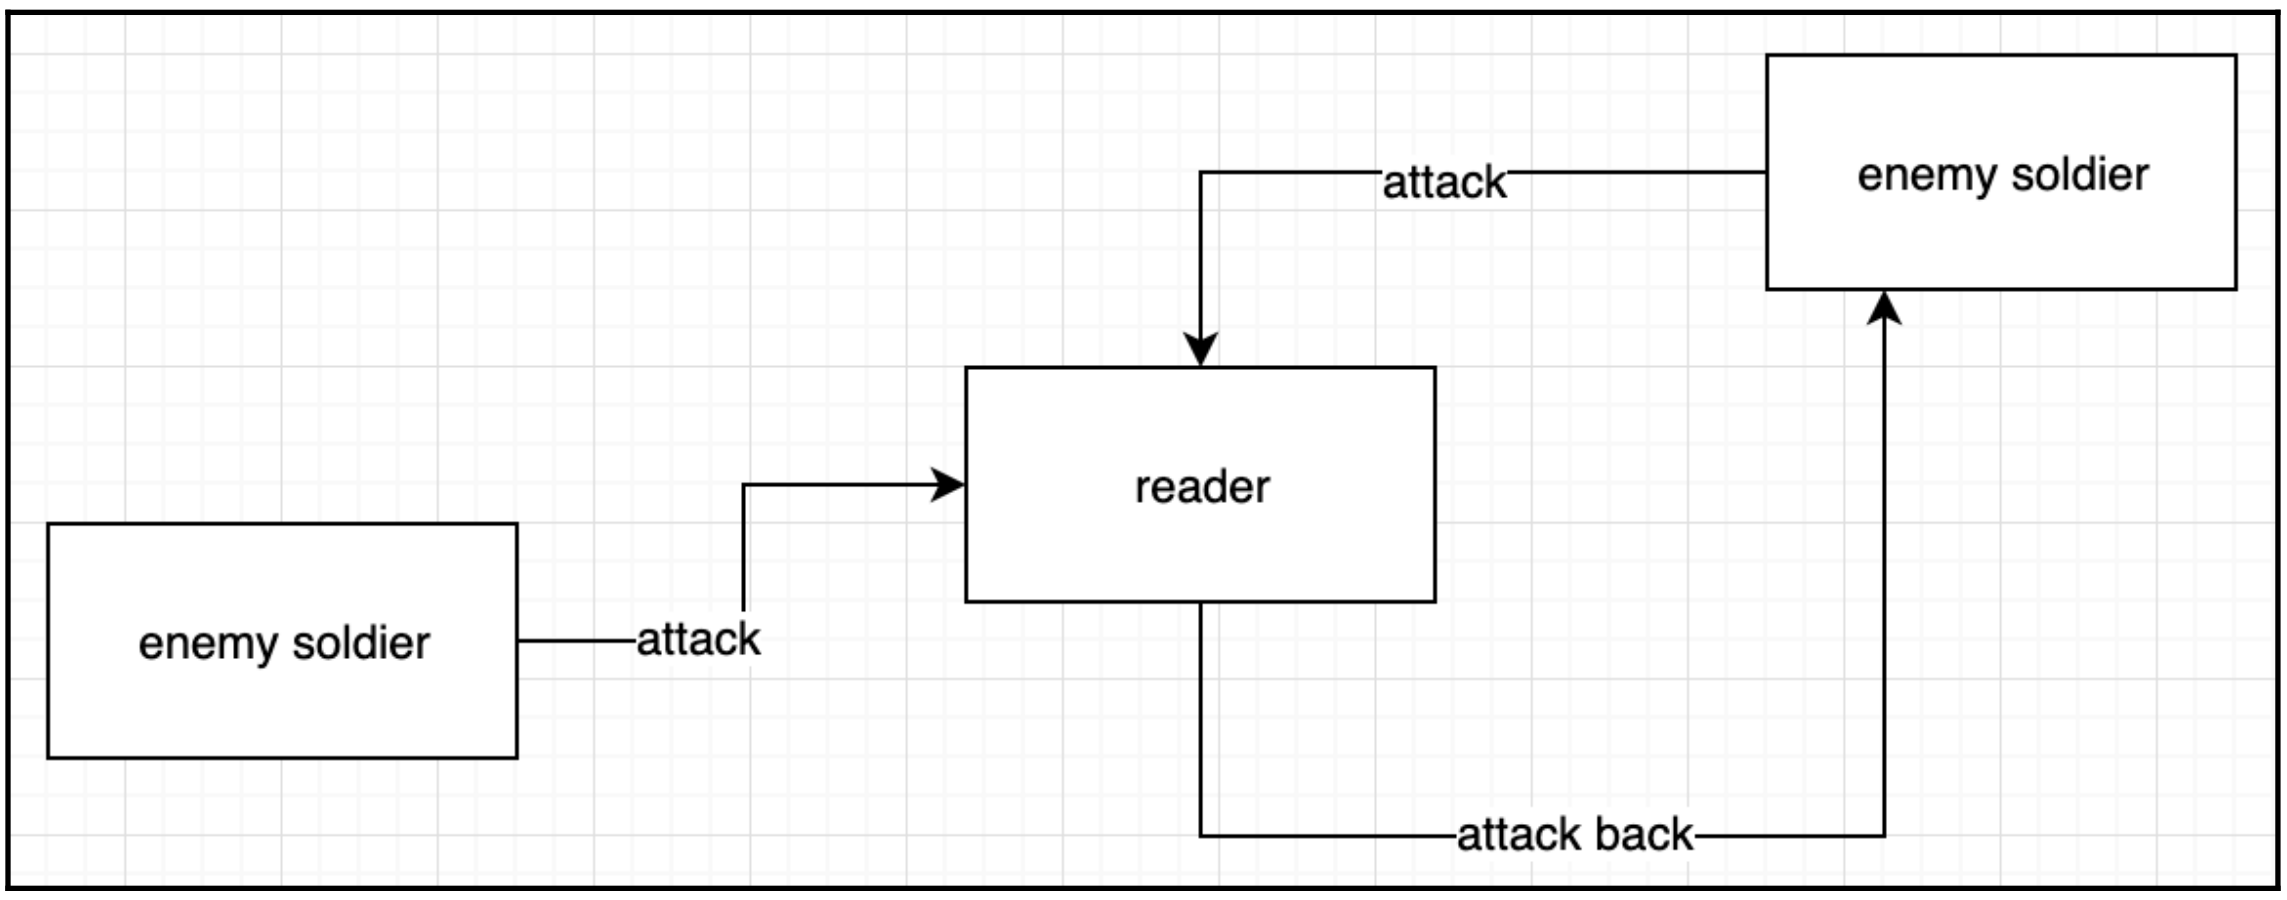
\includegraphics[width=1.0\textwidth]{content/Section-2/Chapter-11/2}
\end{center}

更多的互动发生在游戏中。游戏中有两组,其中一组由玩家控制。另一个是由电脑控制。这意味着作为游戏设计师必须定义敌人。游戏将自动创建读者,并分配给他们创建图书馆、兵营和房屋的任务。每个士兵都应该承担保卫建筑物和读者(人民)的责任。有时,士兵们应该聚在一起,执行攻击任务。 \par
我们将设计一个平台,让玩家创建一个帝国,而游戏也应该创造敌人来完善游戏。玩家将经常面临敌人的攻击,敌人将通过建造更多建筑和生产更多单位而进化。总的来说,我们可以用下图来描述交互: \par

\begin{center}
	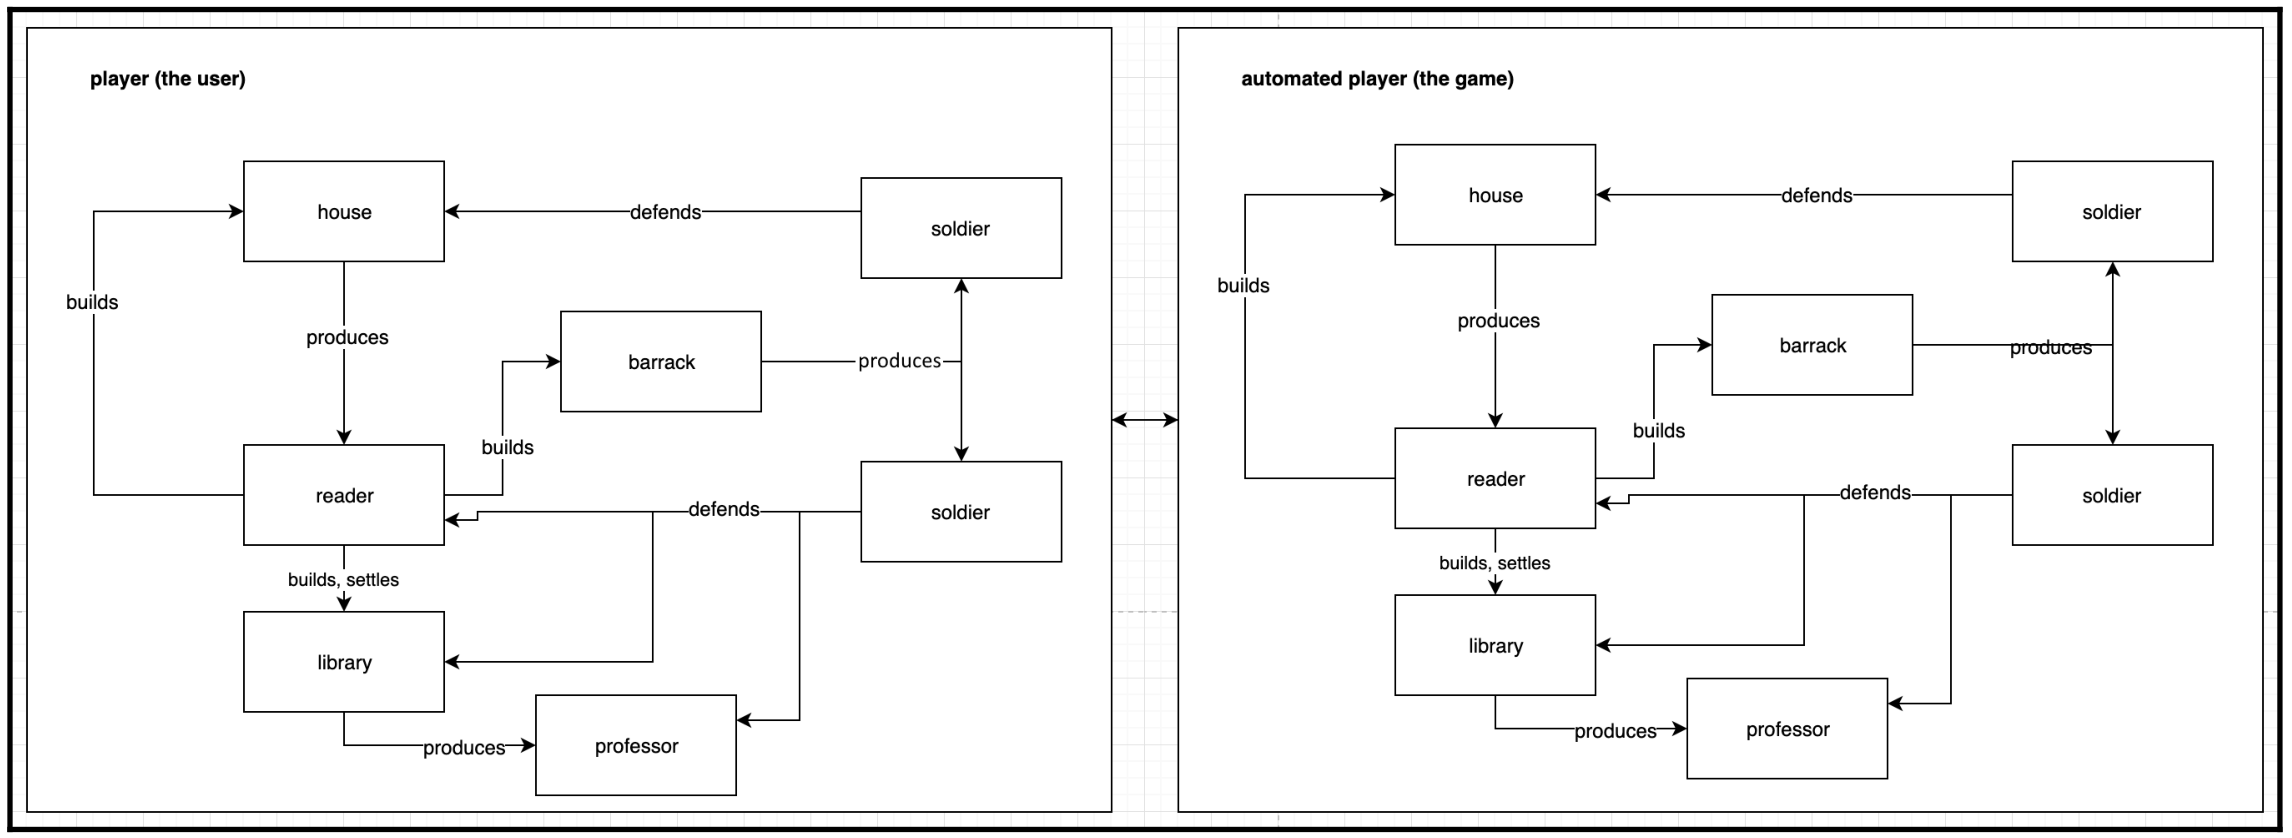
\includegraphics[width=1.0\textwidth]{content/Section-2/Chapter-11/3}
\end{center}

我们将在设计游戏时参考上述图表。 \par

\noindent\textbf{}\ \par
\textbf{设计游戏} \ \par
虽然游戏并不是一款典型的软件,但它的设计却与常规应用设计并无太大区别。我们将从主要实体开始,并将它们进一步分解为类的关系。 \par
在前一节中,我们讨论了游戏组件及其交互作用。我们根据项目开发生命周期进行了需求分析和收集。现在,我们开始设计游戏。 \par

\noindent\textbf{}\ \par
\textbf{设计角色} \ \par
下面的类图代表了一个读者: \par

\begin{center}
	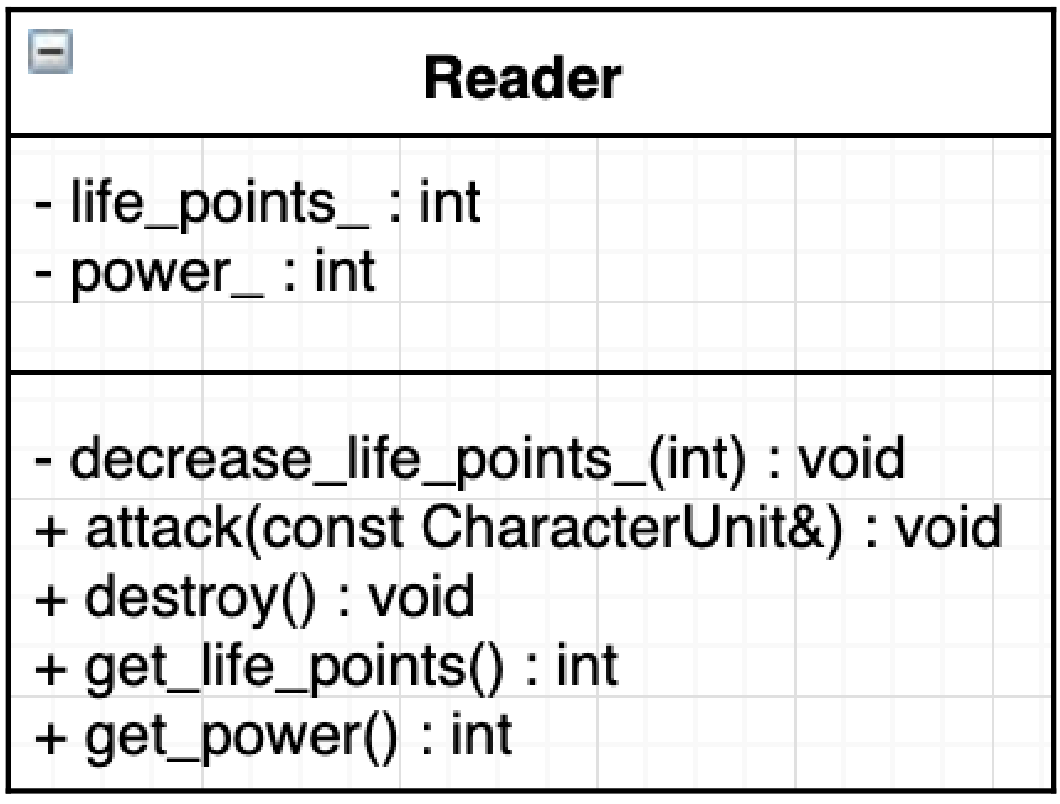
\includegraphics[width=0.6\textwidth]{content/Section-2/Chapter-11/4}
\end{center}

当我们浏览其他角色单位时,我们将为每个角色单位想出一个基类。每个特定的单元将从这个基类继承,并添加特定的属性(如果有的话)。以下是角色单位的完整类图: \par

\begin{center}
	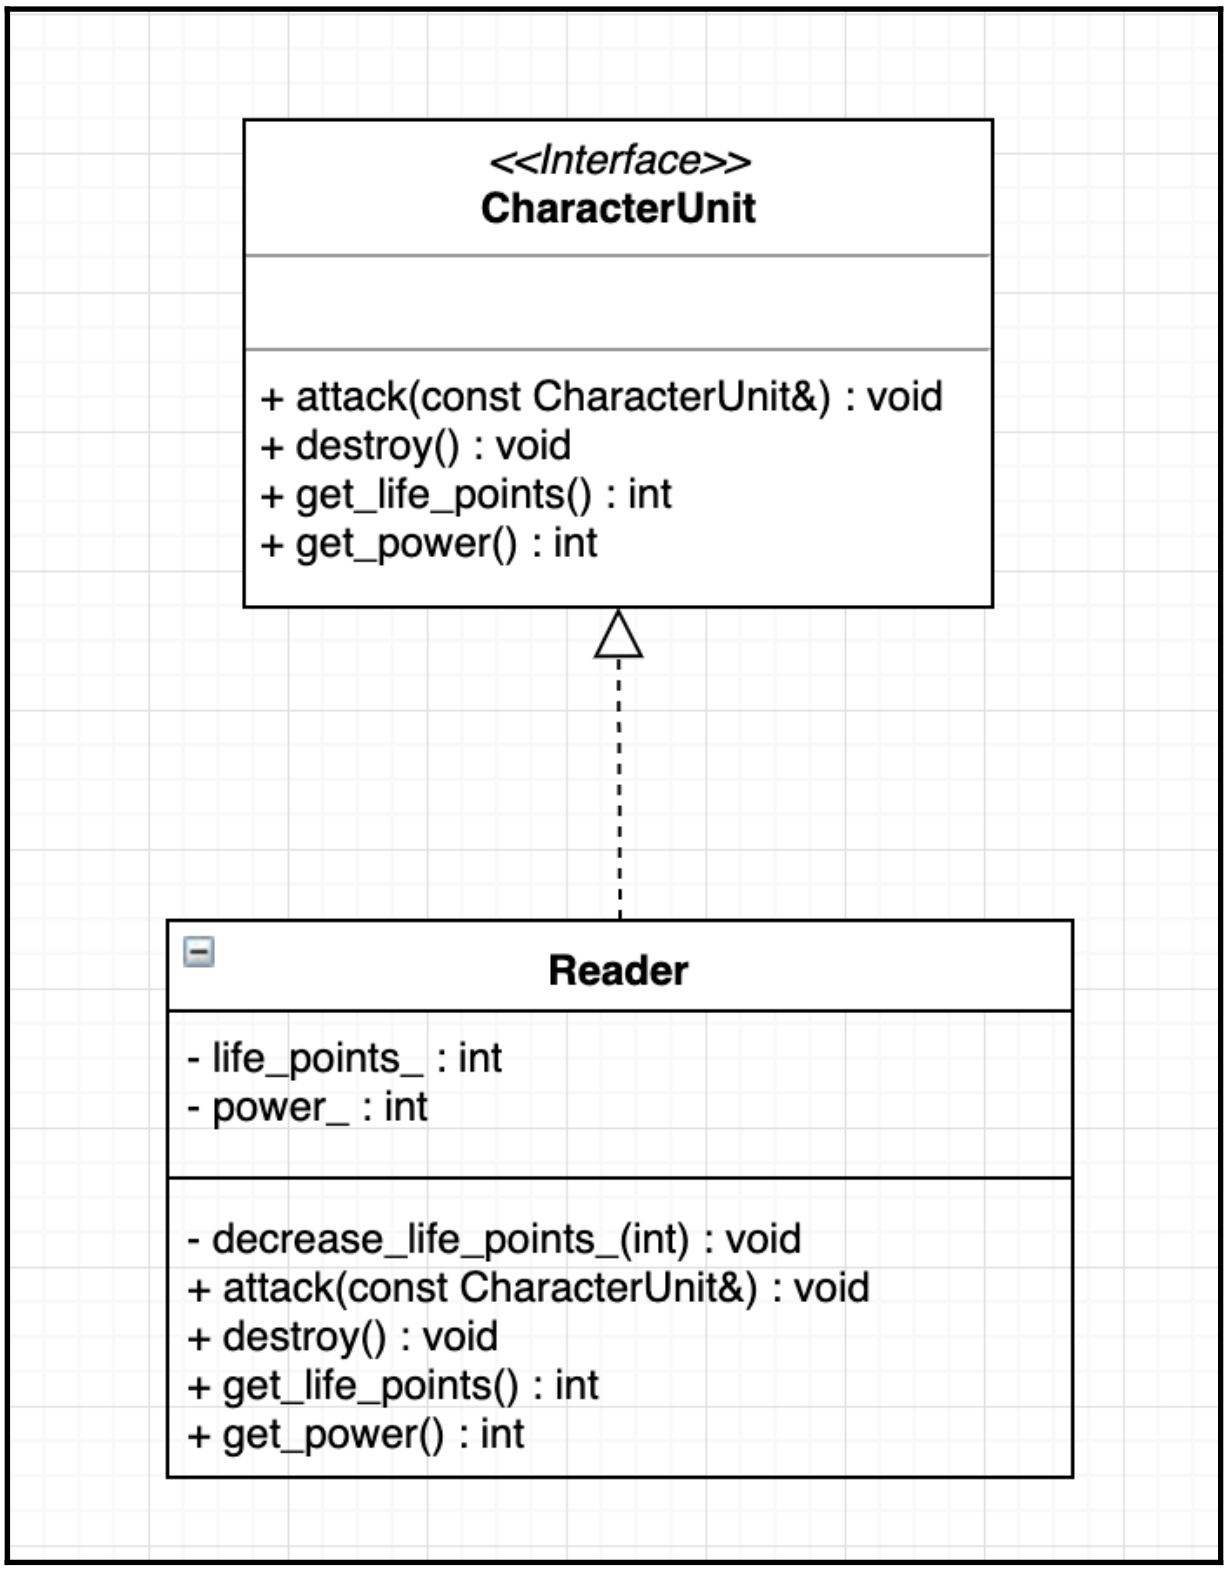
\includegraphics[width=0.8\textwidth]{content/Section-2/Chapter-11/5}
\end{center}

请注意基类——它是一个接口,而不是一个常规类。它定义了在派生类中实现的纯虚函数。以下是CharacterUnit接口在代码中的声明: \par

\begin{lstlisting}[caption={}]
class CharacterUnit
{
public:
	virtual void attack(const CharacterUnit&) = 0;
	virtual void destroy() = 0;
	virtual int get_power() const = 0;
	virtual int get_life_points() const = 0;
};
\end{lstlisting}

attack()会降低角色的生命值,destroy()则会摧毁角色。摧毁不仅意味着将角色从场景中移除,还意味着停止该单位正在进行的所有互动(如建造建筑、自卫等等)。 \par
派生类提供了CharacterUnit接口类的纯虚函数的实现。让我们来看看Reader字符单元的代码: \par

\begin{lstlisting}[caption={}]
class Reader : public CharacterUnit
{
public:
	Reader();
	Reader(const Reader&) = delete;
	Reader& operator=(const Reader&) = delete;
	
public:
	void attack(const CharacterUnit& attacker) override {
		decrease_life_points_by_(attacker.get_power());
	}

	void destroy() override {
		// we will leave this empty for now
	}

	int get_life_points() const override {
		return life_points_;
	}

	int get_power() const override {
		return power_;
	}

private:
	void decrease_life_points_(int num) {
		life_points_ -= num;
		if (life_points_ <= 0) {
			destroy();
		}
	}

private:
	int life_points_;
	int power_;
};
\end{lstlisting}

现在,我们可以通过以下任何一种方式声明Reader: \par

\begin{lstlisting}[caption={}]
Reader reader;
Reader* pr = new Reader();
CharacterUnit* cu = new Reader();
\end{lstlisting}

主要通过基接口类来引用角色单位。 \par

\hspace*{\fill} \\ %插入空行

\includegraphics[width=0.05\textwidth]{images/tip}
请注意复制构造函数和赋值操作符。我们故意把它们标记为删除,因为我们不想通过复制其他单位来创建单位。我们将为该行为使用原型模式。这将在后面讨论。 \par
\noindent\textbf{}\ \par

我们应该为不同类型的单位做同样的事情的场景中,拥有CharacterUnit接口非常重要,例如:我们必须计算两名士兵、一名读者和一名教授对一座建筑造成的全部损害。我们不必保留三个不同的引用来引用三种不同类型的单元,而是将它们都称为CharacterUnits。方法如下: \par

\begin{lstlisting}[caption={}]
int calculate_damage(const std::vector<CharacterUnit*>& units)
{
	return std::reduce(units.begin(), units.end(), 0,
		[](CharacterUnit& u1, CharacterUnit& u2) {
			return u1.get_power() + u2.get_power();
		}
	);
}
\end{lstlisting}

calculate\underline{ }damage()函数对单元类型进行抽象,它不关心读者或士兵。它只调用CharacterUnit接口的get\underline{ }Ppower()方法,该方法保证特定对象的实现。\par
我们将更新角色单位类,让我们继续为建筑设计类。 \par

\noindent\textbf{}\ \par
\textbf{设计建筑} \ \par

\noindent\textbf{}\ \par
\textbf{设计游戏控制器} \ \par

\noindent\textbf{}\ \par
\textbf{游戏事件循环} \ \par

\noindent\textbf{}\ \par
\textbf{使用设计模式} \ \par

\noindent\textbf{}\ \par
\textbf{命令模式} \ \par

\noindent\textbf{}\ \par
\textbf{观察者模式} \ \par

\noindent\textbf{}\ \par
\textbf{享元模式} \ \par

\noindent\textbf{}\ \par
\textbf{原型模式} \ \par

\noindent\textbf{}\ \par
\textbf{设计游戏循环} \ \par

\noindent\textbf{}\ \par
\textbf{总结} \ \par

\noindent\textbf{}\ \par
\textbf{问题} \ \par
\begin{enumerate}
	\item 重写一个私有虚拟函数的目的是什么?
	\item 描述命令设计模式。
	\item 享元模式如何节省内存使用?
	\item 观察者模式和中介模式之间有什么区别?
	\item 为什么我们要将游戏循环设计成一个无限循环?
\end{enumerate}

\noindent\textbf{}\ \par
\textbf{扩展阅读} \ \par
\begin{itemize}
	\item Game Development Patterns and Best Practices: Better games, less hassle by John P.Doran, Matt Casanova:  https:/​/​www.​amazon.​com/​Game-​Development-​Patterns-	Best-​Practices/​dp/​1787127834/​ .
\end{itemize}

\newpage









